\documentclass[dvipdfmx]{jarticle}
\usepackage{graphicx}
\usepackage[top=30truemm,bottom=30truemm,left=25truemm,right=25truemm]{geometry}
\usepackage{listings,jvlisting}

\lstset{
  basicstyle={\ttfamily},
  identifierstyle={\small},
  commentstyle={\smallitshape},
  keywordstyle={\small\bfseries},
  ndkeywordstyle={\small},
  stringstyle={\small\ttfamily},
  frame={tb},
  breaklines=true,
  columns=[l]{fullflexible},
  numbers=left,
  xrightmargin=0zw,
  xleftmargin=3zw,
  numberstyle={\scriptsize},
  stepnumber=1,
  numbersep=1zw,
  lineskip=-0.5ex
}

\begin{document}
\begin{titlepage}
    \begin{center}
        {\huge 情報科学演習C 課題4レポ―ト}
        \vspace{180pt}\\
        \begin{tabular}{rl}
            氏名 & 山久保孝亮\\
            所属 & 大阪大学基礎工学部情報科学科ソフトウェア科学コース\\
            メールアドレス & u327468b@ecs.osaka-u.ac.jp\\
            学籍番号 & 09B22084\\
            提出日 & \today\\
            担当教員 & 平井健士,中島悠太
        \end{tabular}
    \end{center}
\end{titlepage}
\section{課題4-1}
\subsection{プログラムの仕様}
課題4-1で作成したクライアントプログラムchatclient.cの仕様は以下の通りである.
\begin{itemize}
    \item プログラム実行の書式は"chatclient [サーバプログラムを実行中のホスト名] [使用したいユーザ名]"である.
    \item 接続できたかと名前を登録できたかが標準出力に表示される.接続できた場合はチャット機能が使用でき,接続できなかった場合はプログラムが終了する.
    \item チャット機能には以下の3つの機能がある.
    \begin{enumerate}
        \item 標準入力に文字列を書き込んで[Enter]キーを押すと,サーバにその文字列を送信する.
        \item サーバに接続されているほかのホストから送られてきた文字列を受信し,標準入力に表示させる.
        \item EOFを入力するとサーバとの接続が切れ,プログラムを終了する.
    \end{enumerate}
\end{itemize}
また,サーバプログラムchatserver.cの仕様は以下の通りである.
\begin{itemize}
    \item プログラム実行の書式は引数はなしである.
    \item 一度に接続できるユーザの数は5である.
    \item 常に新たなユーザの接続を待っており,接続された場合には接続されたかどうかと,すでに同じユーザ名が登録されていないかを確認し,どちらも
    満たしていればその旨の文字列を送信して新たなユーザとして登録し,いずれかを満たさない場合はその旨の文字列を送信して再び待ち状態に入る.
    \item 登録されたユーザから文字列を受信した場合はその文字列の先頭にユーザ名を追加して送信してきたユーザ以外に追加した後の文字列を送信する.
    \item EOFを受信するとそのユーザの接続を切り,ユーザの情報を削除する.
\end{itemize}
\subsection{クライアントプログラムのアルゴリズム}
今回作成したプログラムは指導書の状態に則って作成しており,以下の図1のフローチャートはそれぞれの状態の遷移の様子を表す.
\begin{figure}[h]
    \centering
    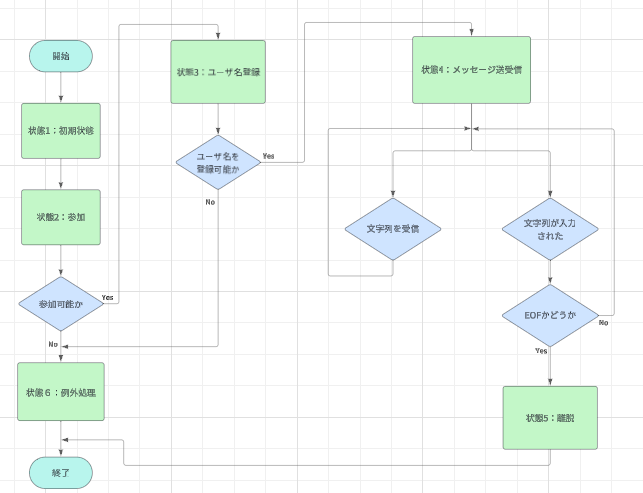
\includegraphics[width=8cm]{4-1clienthurotya.png}
    \caption{クライアントプログラムのフローチャート}
\end{figure}
\subsection{クライアントプログラムの実装方法}
以下の表1はこのプログラムで使用した変数名とその使用法である.
\subsection{サーバプログラムのアルゴリズム}
\subsection{サーバプログラムの実装方法}
\subsection{実行結果}
\section{課題4-2}
\subsection{プログラムの仕様}
\subsection{アルゴリズム}
\subsection{実装方法}
\subsection{実行結果}
\section{考察}
\section{感想}
\section{謝辞}
\section{参考文献}
\end{document}